\documentclass[a4paper, 12pt]{article} % A4 paper size, default 11pt font size and oneside for equal margins


\usepackage[utf8]{inputenc} % Required for inputting international characters
\usepackage[spanish]{babel}
\usepackage[T1]{fontenc} % Output font encoding for international characters
\usepackage{graphicx}
\usepackage{amsmath}
\usepackage{amsthm} % para teoremas y deficiones
\usepackage{tikz}
\usepackage{float}
\usepackage{verbatim}
\parskip=1mm % espacio entre parrafos
\newtheorem*{mydef1}{Definición} %para las definiciones

%----------------------------------------------------------------------------------------
%	TITLE PAGE
%----------------------------------------------------------------------------------------

\begin{document}

\newpage
\begin{titlepage}

	\centering % Centre everything on the title page

	\scshape % Use small caps for all text on the title page

	\vspace*{\baselineskip} % White space at the top of the page

	%------------------------------------------------
	%	Title
	%------------------------------------------------

	\rule{\textwidth}{1.6pt}\vspace*{-\baselineskip}\vspace*{2pt} % Thick horizontal rule
	\rule{\textwidth}{0.4pt} % Thin horizontal rule

	\vspace{0.75\baselineskip} % Whitespace above the title

	{\LARGE Funciones Hash\\y\\Integridad de Datos\\} % Title

	\vspace{0.75\baselineskip} % Whitespace below the title

	\rule{\textwidth}{0.4pt}\vspace*{-\baselineskip}\vspace{3.2pt} % Thin horizontal rule
	\rule{\textwidth}{1.6pt} % Thick horizontal rule

	\vspace{2\baselineskip} % Whitespace after the title block

	%------------------------------------------------
	%	Subtitle
	%------------------------------------------------

	Trabajo para la la asignatura 'Modelos de Computación' de Ingeniería Informática.

	\vspace*{3\baselineskip} % Whitespace under the subtitle

	%------------------------------------------------
	%	Editor(s)
	%------------------------------------------------

	Realizado por

	\vspace{0.5\baselineskip} % Whitespace before the editors

	{\scshape\Large Aarón Arias Pérez\\} % Editor list

	\vspace{0.5\baselineskip} % Whitespace below the editor list

	\textit{Universidad de Cádiz} % Editor affiliation

\end{titlepage}

%----------------------------------------------------------------------------------------


\newpage

\tableofcontents

\listoffigures

\newpage

\section{Introducción}
Las funciones criptográficas hash juegan un papel fundamental en la criptografía
moderna. Nuestro enfoque está restringido al uso de las funciones hash para Integridad
de datos y autentificación de mensajes.

Las funciones hash toman un mensaje como entrada y produce una salida llamada hash-code,
o simplemente hash. En concreto, una función hash $h$ nos convierte una cadena de una
longitud cualquiera a una cadena de tamaño fijo.

Para un dominio $D$ y un rango $R$ con $h: D \rightarrow R$ y $|D| > |R|$, la función nos puede dar salidas iguales
para entradas distintas y esto es inevitable.
Si restringimos $h$ al dominio de t-bit entradas ($t>n$, siendo n el tamaño fijo de la cadena),
si $h$ fuera aleatorio en el sentido de que todas las salidas fueran esencialmente equiprobables,
tendríamos alrededor de $2^{t-n}$ posibles entradas para cada salida, y dos entradas escogidas
aleatoriamente podrían tener la misma salida con probabilidad $2^{-n}$.
La idea básica de las funciones hash es que un hash-value sirve como una imagen representativa
compacta de una cadena de entrada, y puede ser usada como si fuera únicamente identificable con
esa cadena.

Las funciones hash se usan para integridad de datos junto con esquemas de firma digital, donde
por varias razones un mensaje normalmente es hasheado (hashed) primero, y luego el hash-value,
como un mensaje representativo, es firmado en el mensaje original.
Una clase distinta de funciones hash, llamadas MACs (message authentication codes), permiten la
autentificación de mensajes mediante técnicas simétricas.
Los algoritmos MAC se pueden interpretar como funciones hash que toman dos entradas funcionales
distintas, un mensaje y una clave secreta, y produce una salida de tamaño fijo (n bit), con
el objetivo de que sea prácticamente inviable producir la misma salida sin conocer la clave.
Los MACs pueden ser usados para proveer integridad de datos y autentificación de origen de
datos simétricos, así como la identificación en esquemas de clave simétrica.

\newpage
\begin{figure}[h!]
	    \centering
	    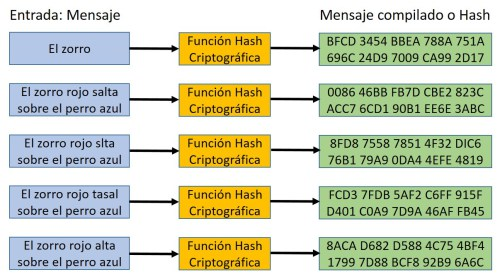
\includegraphics[width=1\textwidth]{imagen_intro.jpg}
	    \caption{Ejemplos de hashing}
	    \label{fig:Ejemplos_hashing}
\end{figure}

Un uso típico de funciones hash sin clave para integridad de datos es el siguiente. El hash-value
correspondiente a un mensaje 'x' es computado en tiempo T1. La integridad de este hash-value
(pero no el mensaje en si mismo) es protegida de alguna forma. En un momento posterior T2, se
lleva a cabo la siguiente prueba para comprobar si el mensaje ha sido alterado. El problema
de preservar la integridad de un mensaje potencialmente grande es así reducida a un hash-value
pequeño. Dado que la existencia de colisiones está garantizada en asignaciones de muchos a uno
(many-to-one), la asociación única entre las entradas y los hash-value puede ser, en el mejor
de los casos, de sentido computacional. Un hash-value debería ser identificable únicamente con
una sola entrada, y las colisiones deberían ser computacionalmente díficiles de encontrar (no
debería ocurrir nunca en la pŕactica).

\newpage
\section{Clasificación}
Al nivel mas alto, las funciones hash pueden agruparse en dos clases: unkeyed hash functions,
cuya especificación dicta que solo haya un parámetro de entrada (un mensaje); y keyed
hash functions, cuya especificación dicta que haya dos entradas, un mensaje y una clave secreta.

\begin{mydef1}
Una función hash es una función $h$ la cual tiene como mínimo las siguientes dos
propiedades:\\ 1) Compresión. La función $h$ asigna una entrada $x$ de tamaño arbitrario a una
salida $h(x)$ de un tamaño fijado n.\\
2) Facilidad de cálculo. Dado $h$ y una entrada $x$, $h(x)$ es fácil de computar.
\end{mydef1}

Como se ha definido aquí, una función hash implica una función hash 'unkeyed'. A veces
cuando el tratamiento es a un nivel general, este término es abusado de alguna manera
para que se use tanto como para funciones hash 'keyed' como 'unkeyed'.

1) MDCs (modification detection codes).
El propósito de un MDC es proveer una imagen representativa (o hash) de un mensaje, satisfaciendo
las propiedades adicionales que se muestran a continuación. El objetivo final es facilitar,
junto con mecanismos adicionales, las garantías de la integridad de datos que son requeridas por
las aplicaciones específicas. Los MDCs son una subclase de funciones hash unkeyed. Algunas de
las clases específicas de MDCs son:\\
1) OWHFs (one-way hash functions). Para estos, encontrar una entrada que codifique en un hash-value
pre-especificado es díficil.\\
2) CRHFs (collision resistant hash functions). Para estos, encontrar dos entradas que tengan el
mismo hash-value es díficil.

2) MACs (message authentication codes).
El propósito de un MAC es facilitar, sin el uso de mecanismos adicionales, las garantías sobre el
origen del mensaje y su integridad. Los MACs tienen dos parámetros funcionales distintos, un
mensaje de entrada y una clave secreta. Son una subclase de funciones hash 'keyed'.

En la \textit{figura 2} se muestra un esquema de la clasificación de las funciones hash.
\newpage
\begin{figure}[h!]
\begin{tikzpicture}[sibling distance=10em,
  every node/.style = {shape=rectangle, rounded corners,
    draw, align=center,
    top color=white, bottom color=green!20}]]
  \node {Hash functions}
  	child { node {unkeyed}
			child { node {MDCs}
				child { node {OWHF} }
				child { node {CRHF} }}
			child { node {other applications}}}
    child { node {keyed}
      child { node {other applications}}
      child { node {MACs} } };
\end{tikzpicture}
\caption{Clasificacion funciones hash.}
\end{figure}

En general, se supone que la especificación algorítmica de una función hash es de conocimiento
público. Por lo tanto, en el caso de los MDCs, dado un mensaje como entrada, cualquiera
puede calcular el hash-value. En el caso de los MACs, dado un mensaje como entrada, cualquier
persona con conocimiento de la clave puede calcular el hash-value.

\subsection{Propiedades básicas}
Tres propiedades potenciales (a parte de la facilidad de cómputo y la compresión), para funciones
hash 'unkeyed' $h$ con entradas $x$, $x'$ y salidas $y$, $y'$.

\textbf{1) Resistencia a la preimagen.} Para esencialmente todas las salidas pre-especificadas, no es factible
computacionalmente encontrar cualquier entrada que codifique a esa salida. Ejemplo: para encontrar
cualquier preimagen $x'$ tal que $h(x') = y$ cuando dado un $y$ para la cual no se
conoce una entrada correspondiente.

\textbf{2) Resistencia a la 2ª-preimagen.} No es computacionalmente factible encontrar cualquier segunda entrada
que tenga la misma salida. Ejemplo: dado $x$, encontrar una
2ª-preimagen $x' \neq x$ tal que $h(x)=h(x')$.

\textbf{3) Resistencia a la colisión.} No es computacionalmente factible encontrar cualquiera dos entradas
distintas $x$, $x'$ que codifiquen en la misma salida. Ejemplo: para cada $h(x) = h(x')$.

No se ha definido nada sobre lo computacionalmente no-factible y dificultad de cómputo, porque son
términos relativos. Se puede considerar la facilidad de cómputo cuando se trata de uso de espacio y
tiempo polinomiales. La infactibilidad computacional se da cuando es muy costoso el cómputo y puede
que con los recursos disponibles sea inabordable.

\newpage
\subsection{Propiedades hash requeridas para aplicaciones específicas}
A causa de que puede haber costes asociados con propiedades específicas, los CRHFs son en general
mas dificiles de construir que los OWHFs y tienen hash-values aproximadamente del doble de tamaño.
Eso debe entenderse como qué propiedades son realmente necesarias para aplicaciones particulares y
por qué lo son. Las técnicas seleccionadas mediante las cuales las funciones hash se usan para
la integridad de los datos, y las propiedades correspondientes requeridas por estas aplicaciones,
se resumen en la \textit{figura 3}.

En general, un MDC deberia ser un CRHF si una parte no confiable tiene control sobre el contenido
de la entrada de la función hash. Un OWHF es suficiente, incluyendo el caso donde solo hay una
parte involucrada (por ejemplo, una aplicación de almacenamiento y recuperación).
El control sobre el formato preciso de las entradas se puede eliminar introduciendo aleatoriedad
que es incontrolable por una o ambas partes. Sin embargo, hay que tener en cuenta que las técnicas
de integridad de datos basadas en una clave secreta compartida generalmente implican confianza
mutua y no abordan la no repudiación. En este caso, la resistencia a la colisión puede (o no) ser
un requisito.

\restylefloat{table}
\begin{figure}[h!]
	\begin{table}[H]
	\centering
	\label{tabla_1}
	\begin{tabular}{lcccl}
	\begin{tabular}[c]{@{}l@{}}Propiedades hash requeridas $\rightarrow$\\ Aplicación $\downarrow$\end{tabular} & \begin{tabular}[c]{@{}c@{}}resistencia a la\\ preimagen\end{tabular} & \begin{tabular}[c]{@{}c@{}}2ª preimagen\end{tabular} & \begin{tabular}[c]{@{}c@{}}resistencia a\\ colisiones\end{tabular} &  \\
	MDC + asymmetric signature                                                                                  & yes                                                                  & yes                              & yes*                                                               &  \\
	MDC + authentic channel                                                                                     &                                                                      & yes                              & yes*                                                               &  \\
	MDC + symmetric encryption                                                                                  &                                                                      &                                  &                                                                    &  \\
	hash for one-way password file                                                                              & yes                                                                  &                                  &                                                                    &  \\
	MAC (clave desconocida por el atacante)                                                                     & yes                                                                  & yes                              & yes*                                                               &  \\
	MAC (clave conocida por el atacante)                                                                        &                                                                      & yes**                            &                                                                    &
	\end{tabular}
	\end{table}
	\caption{Propiedades de resistencia requeridas para aplicaciones con integridad de datos especificadas.}
\end{figure}
\textbf{*:} Se requiere resistencia si el atacante puede montar un \textit{chosen message attack}.\\

\textbf{**:} Se requiere resistencia en casos excepcionales de autenticación de varios niveles.

\newpage
\subsection{Otras propiedades y aplicaciones.}
La mayoría de las funciones hash 'unkeyed' comunes que encontramos, en la práctica fueron
originalmente diseñadas con el propósito de proveer integridad de datos, incluyendo la toma
digital de huellas dactilares de los mensajes junto con firmas digitales. De hecho, la mayoría
de ellos son MDCs diseñados para tener las propiedades de preimagen, 2ª-preimagen o resistencia
de colisiones.

En general, el uso de funciones hash para otros propósitos para los que no fueron diseñados
requieren de propiedades adicionales que no nos proveen estas funciones por como fueron diseñadas.
Sin embargo, se han propuesto funciones hash 'unkeyed' que tienen propiedades asociadas con
funciones one-way para una amplia gama de aplicaciones:

\textbf{1) Derivación de clave.} Para computar secuencias de nuevas claves provenientes de claves anteriores.
Un primer ejemplo es la derivación de clave en terminales POS (point-of-sale). Aquí un requisito
importante es que el compromiso de las claves actualmente activas no debe comprometer la seguridad
de las claves de transacciones anteriores. Un segundo ejemplo es en la generación de secuencias
de contraseña de un solo uso basadas en funciones one-way.

\textbf{2) Generación de números pseudo-aleatorios.} Para generar secuencias de números que tienen varias
propiedades de aleatoriedad. Debido a la dificultad de generar números pseudo-aleatorios
criptográficamente fuertes, los MDCs no deberían ser usados para este propósito a menos que los
requisitos de aleatoriedad se entiendan claramente, y el MDC se verifique para satisfacerlo.

\newpage
\section{Construcciones básicas}
\subsection{Modelo general para funciones hash iteradas.}
La mayoría de las funciones hash 'unkeyed' $h$ están diseñadas como procesos iterativos que modifica
las entradas de longitud arbitraria procesando sucesivos bloques de tamaño fijo de la entrada, como
se puede ver en la \textit{figura 4}.

\begin{figure}[h!]
	\centering
	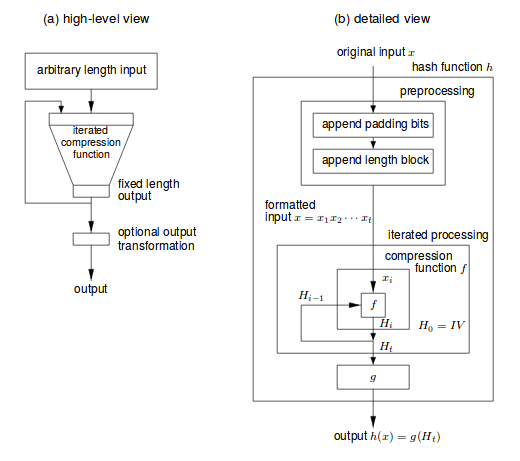
\includegraphics[width=1\textwidth]{imagen_hashfunction.png}
	\caption{Modelo general para funciones hash iteradas.}
	\label{fig:Modelo_iteradas}
\end{figure}

Una entrada hash $x$ de longitud finita arbitraria es dividida en bloques \textit{r-bit} $x_i$ de tamaño fijo.
Este preprocesamiento generalmente implica la adición de bits adicionales (de relleno) según sea
necesario para lograr una longitud de bits general, que es un múltiplo de la longitud del bloque \textit{r}, y
a menudo incluye un bloque o bloque parcial que indica la longitud de bit de la entrada sin relleno.
Cada bloque $x_i$ sirve entonces como entrada para una función hash interna $f$ de tamaño fijo, la función
de compresión de $h$, que calcula un nuevo resultado intermedio de longitud n-bit para algunos n fijos,
como una función del resultado intermedio previo de n bits y el siguiente bloque de entrada $x_i$.

Tomando como $H_i$ el resultado parcial después de la etapa $i$, el proceso general para una función
hash iterada con entrada $x = x_1 x_2 ... x_t$, puede ser modelada de la siguiente forma:
\begin{equation*}
	H_o = IV;  H_i = f(H_{i-1}, x_i),  1 \leq i \leq t;  h(x) = g(H_t).
\end{equation*}
$H_{i-1}$ sirve como la variable de encadenamiento de n-bits entre la etapa $i-1$ y la etapa $i$, y
$H_o$ es un valor inicial pre-definido o un valor de inicialización (IV). Una transformación de salida opcional
$g$ (ver \textit{figura 4}) se usa en un paso final para asignar la variable de encadenamiento de n-bit a
un resultado m-bit $g(H_t)$; $g$ es a menudo el mapeo de identidad $g(H_t) = H_t$.

Las funciones hash particulares se distinguen por la naturaleza del preprocesamiento, la función de compresión y
la transformación de salida.

\subsection{Tamaños de bit requeridos para una seguridad práctica.}
Suponer que una función hash produce hash-values de n-bits, y como un \textit{benchmark} representativo, asumimos
que $2^{80}$ (pero no menos) operaciones son aceptablemente factible de computar. Entonces las siguientes
declaraciones se pueden hacer con respecto a n.\\ \\
1) Para un OWHF, se requiere $n \geq 80$. Los ataques exhaustivos \textit{offline} requieren como máximo $2^n$
operaciones; esto se puede reducir con precomputación.\\ \\
2) Para un CRHF, se requiere $n \geq 160$. Los ataques \textit{birthday} se pueden aplicar.

\newpage

3) Para un MAC, con $n \geq 64$ junto con una clave MAC de 64-80 bits, es suficiente para la mayoría
de las aplicaciones y entornos. Si una sola clave MAC permanece en uso, los ataques \textit{offline} pueden
ser posibles dado uno o más pares de textos MAC; pero para un algoritmo MAC apropiado, la resistencia a la preimagen
y a la 2ª-preimagen (tanto como la resistencia a la colisión) debe seguir directamente del desconocimiento de la
clave, y por lo tanto la seguridad con respecto a dichos ataques debe depender del tamaño de la clave en lugar de n.

Para ataques que requieren consultas \textit{online}, se deben usar controles adicionales para limitar el número
de cada consulta, restringir el formato de las entradas MAC, o evitar la divulgación de las salidas MAC para
entradas aleatorias.

Con controles especiales, valores tan pequeños como $n=32$ o $40$ pueden ser aceptables; pero
se recomienda precaución, ya que incluso con claves MAC one-way, la posibilidad de adivinar cualquier MAC al azar es
de $2^{-n}$, y los factores relevantes son el número total de intentos a los que está sujeto un sistema a lo
largo de su vida, y las consecuencias de obtener una falsificación exitosa.


\newpage
\section{Integridad de datos y autenticación de mensajes}
Esta sección considera el uso de funciones hash para la integridad de datos y la autenticación de mensajes,
a partir de definiciones en el contexto.

\subsection{Trasfondo y definiciones.}
Esta subsección discute la integridad de datos, la autenticación del origen de datos (autenticación de mensajes),
y la autenticación de transacciones.

Por lo general, se requieren garantías de que los datos provengan realmente de su fuente acreditada (autenticación
del origen de los datos) y que su estado no haya sido alterado (integridad de datos).
Estos problemas no pueden separarse; los datos que han sido alterados de manera efectiva tienen una nueva fuente;
y si no se puede determinar una fuente, entonces el problema de la alteración no se puede resolver (sin referencia
a una fuente). Los mecanismos de integridad proporcionan implícitamente la autenticación del origen de datos, y
viceversa.

\subsubsection{Integridad de datos.}

\begin{mydef1}
La integridad de datos es la propiedad por la cual los datos no han sido alterados de manera no autorizada desde
el momento en el que fueron creados, transmitidos o almacenados por una fuente autorizada.
\end{mydef1}

La verificación de la integridad de datos requiere que solo un subconjunto de todos los elementos de datos
candidatos satisfaga los criterios particulares que distinguen lo aceptable de lo inaceptable. Los criterios
que permiten reconocer la integridad de los datos incluyen una redundancia o expectativa adecuada con
respecto al formato. Las técnicas criptográficas para la integridad de los datos se basan en información
secreta o canales auténticos.

El foco específico de la integridad de los datos está en la composición de datos a nivel de bit. Las operaciones
que invalidan la integridad incluyen: inserción de bits, incluyendo ítems de datos completamente nuevos de
fuentes fraudulentas; eliminación de bits (excepto la eliminación de elementos de datos completos); reordenamiento
de bits o grupos de bits; inversión o sustitución de bits; y cualquier combinación de estos, como el ensamblaje
de mensajes (reutilización de subcadenas adecuadas para construir elementos de datos nuevos o alterados).

La integridad de los datos incluye la noción de que los elementos de datos están completos. Para los artículos
divididos en bloques múltiples, las alteraciones anteriores se aplican análogamente a los bloques visualizados
como subcadenas de una cadena de datos contigua.

\subsubsection{Autenticación del origen de datos (autenticación de mensaje).}

\begin{mydef1}
La \textit{autenticación del origen de datos} es un tipo de autenticación mediante el cual una parte se corrobora
como la fuente (original) de datos específicos creados en algún momento (generalmente inespecificado).
\end{mydef1}

Por definición, la autenticación del origen de datos incluye la integridad de los datos.

\begin{mydef1}
La \textit{autenticación de mensaje} es un término usado análogamente con la autenticación del origen de datos.
Provee autenticación del origen de datos con respecto a la fuente original del mensaje (y integridad de datos,
pero no hay garantías de exclusividad y puntualidad).
\end{mydef1}

Los métodos usados para proveer autenticación del origen de datos incluyen los siguientes:\\
1. MACs.\\
2. esquemas de firma digital.\\
3. anexando un valor secreto (antes de la encriptación) de autenticador al texto encriptado.

\subsubsection{Autenticación de transacción.}

\begin{mydef1}
La \textit{autenticación de transacción} denota autenticación de mensaje aumentada, para proporcionar adicionalmente
garantías de exclusividad y puntualidad en los datos (evitando así la repetición indetectable de los mensajes).
\end{mydef1}

\newpage
Generalmente se brindan las garantías de exclusividad y puntualidad de la definición anterior mediante el uso
apropiado de parámetros variantes de tiempo (TVP). Estos incluyen números aleatorios en protocolos de
desafío-respuesta, números de secuencia, y marcas de tiempo. Esto puede verse como una combinación de autenticación
de mensaje y autenticación de entidad. En términos generales,

\begin{equation*}
\text{autenticación de mensaje} + TVP = \text{autenticación de transacción}
\end{equation*}

\restylefloat{table}
\begin{figure}[h!]
	\begin{table}[H]
	\centering
	\label{tabla_2}
	\begin{tabular}{lcccl}
	\begin{tabular}[c]{@{}l@{}}Propiedades $\rightarrow$\\ Tipo de autenticación $\downarrow$\end{tabular} & \begin{tabular}[c]{@{}c@{}}identificación\\ de fuente\end{tabular} & \begin{tabular}[c]{@{}c@{}}integridad\\ de datos\end{tabular} & \begin{tabular}[c]{@{}c@{}}puntualidad o\\ exclusividad\end{tabular} &  \\
	autenticación de mensaje                                                                                 & yes                                                                  & yes                              & ---                                                               &  \\
	autenticación de transacción                                                                                    & yes                                                                     & yes                              & yes                                                              &  \\
	autenticación de entidad                                                                                 & yes                                                                      & ---                                & yes                                                                   &  \\
	autenticación de clave                                                                             & yes                                                                  & yes                                 & deseable                                                                   &  \\                                                                       &
	\end{tabular}
	\end{table}
	\caption{Propiedades de varios tipos de autenticación.}
\end{figure}


\newpage

\nocite{*} %para que se incluya la bibliografia
\bibliography{biblio}
\bibliographystyle{ieeetr}

\end{document}
